\documentclass[11.5pt]{article}
\usepackage[a4paper, margin=0.75in]{geometry}
%\usepackage[myheadings]{fullpage}
\usepackage{fancyhdr}
\usepackage{lastpage}
\usepackage{graphicx, wrapfig, subcaption, setspace, booktabs}
\usepackage[T1]{fontenc}
\usepackage[font=small, labelfont=bf]{caption}
\usepackage{fourier}
\usepackage[protrusion=true, expansion=true]{microtype}
\usepackage[english]{babel}
\usepackage{sectsty}
\usepackage{url, lipsum}
\usepackage{tgbonum}
\usepackage{hyperref}
\usepackage{xcolor}
\usepackage{pdfpages}
\newcommand{\HRule}[1]{\rule{\linewidth}{#1}}
\onehalfspacing
\setcounter{tocdepth}{5}
\setcounter{secnumdepth}{5}
\sectionfont{\scshape}





\begin{document}
{\fontfamily{cmr}\selectfont
\title{ \normalsize 
        \textsc{} 
        \vspace{0.5cm}
		\HRule{0.5pt} 
		\LARGE \textbf{\uppercase{Mechatronics Final Report}
		\HRule{0.5pt} 
		\vspace{0.5cm}}
		}
}

\date{December 15, 2019}

\author{
		Sirena DePue, Grace Ding, Marigot Fackenthal \\
		Group 47 \\
		Cornell University \\
		MAE 3780 | Fall 2019
		} 

\maketitle

\newpage
\tableofcontents
\listoffigures





\newpage
\section{Introduction}
\noindent
As the grand finale to our semester of MAE 3780, we showed off our newfound skills in a class-wide autonomous robot competition. The objective of the competition this year was to collect small blocks from the middle of an arena and bring them to an assigned side. After one minute, the robot with the most blocks on its side was proclaimed the victor.
\\*

\noindent
This report serves as the complete documentation for our robot, ``Grover.'' It includes an overview of the mechanical design and strategy, our strengths and weaknesses, and future improvements. 



\section{Mechanical Design}
\subsection{Overview}

\noindent
\textit{Block collection:}   The front of our robot featured a rigid plow as a first-order means of collecting blocks. It was made of three main panels, each of which were laser cut with interlocking finger joints. All exposed surfaces of the plow were then covered in bubbles of duct tape, ensuring that blocks we contacted remained in our control throughout gameplay. Tape-covered extrusions were attached to the sides of the robot for the same purpose. These extrusions were made of cardboard, since their robustness was not essential to our strategy.
\\*

\noindent
\textit{Sensor mounts:}    Three small QTI mounts were added to the bottom of the plow. This was done after repeated attempts to fasten the sensors with tape, all of which resulted in false readings triggered by inconsistent heights. By laser cutting the QTI mounts, we were able to precisely position the sensors without the risk of their heights being accidentally altered during matches. 


\subsection{CAD Render and Drawing}

\begin{center}
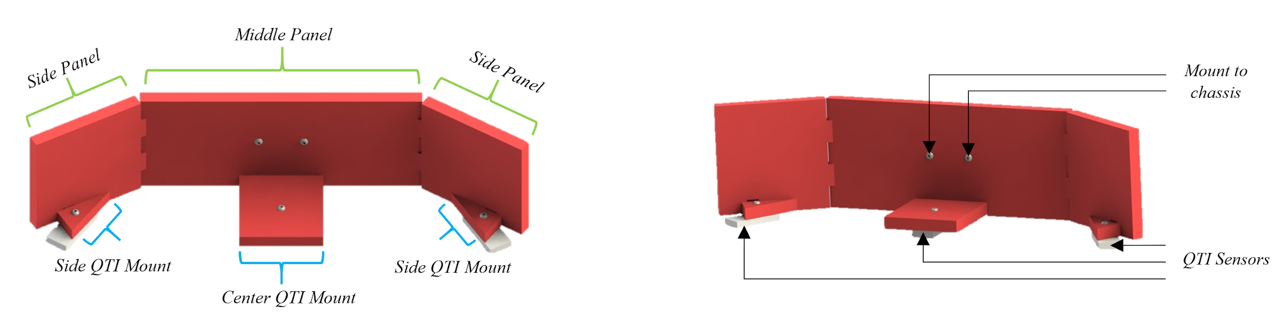
\includegraphics[scale=1.8]{Images/CADrenders}
\captionof{figure}{\textit{CAD Renders}}
\end{center}

\begin{center}
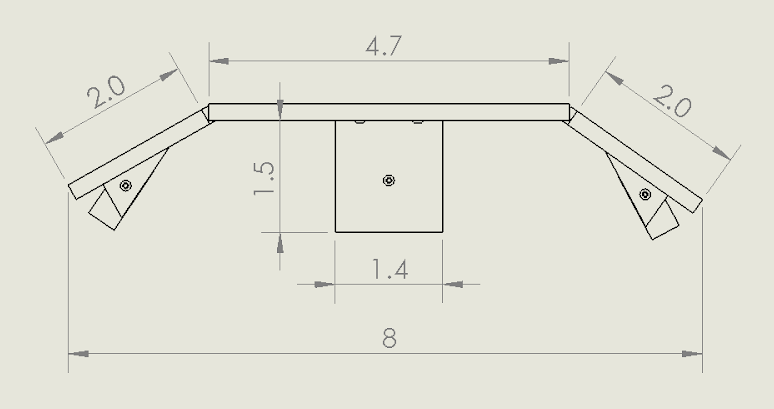
\includegraphics[scale=0.4]{Images/CADdrawing}
\captionof{figure}{\textit{Drawing | Basic Dimensions (Inches)}}
\end{center}


\subsection{Final Product}

\begin{center}
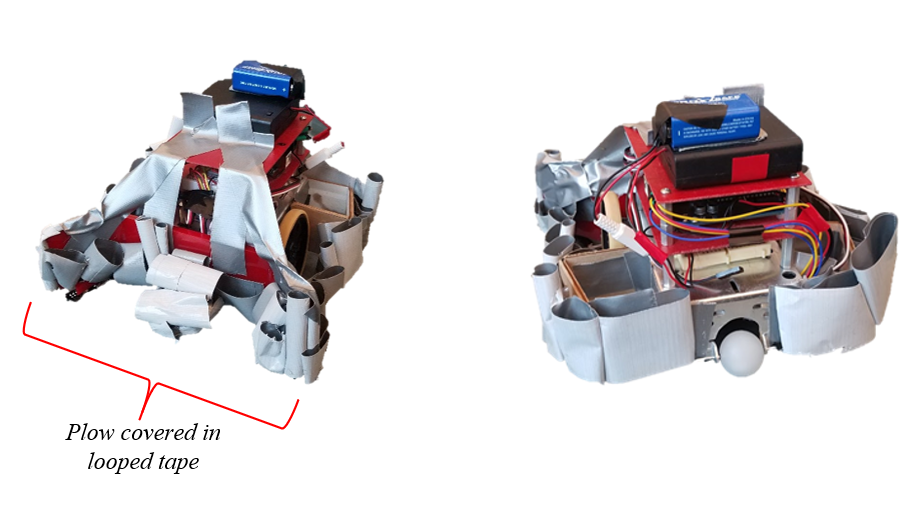
\includegraphics[scale=2]{Images/product1}
\captionof{figure}{\textit{Build Diagrams | Front View (L), Back View (R)}}
\end{center}

\begin{center}
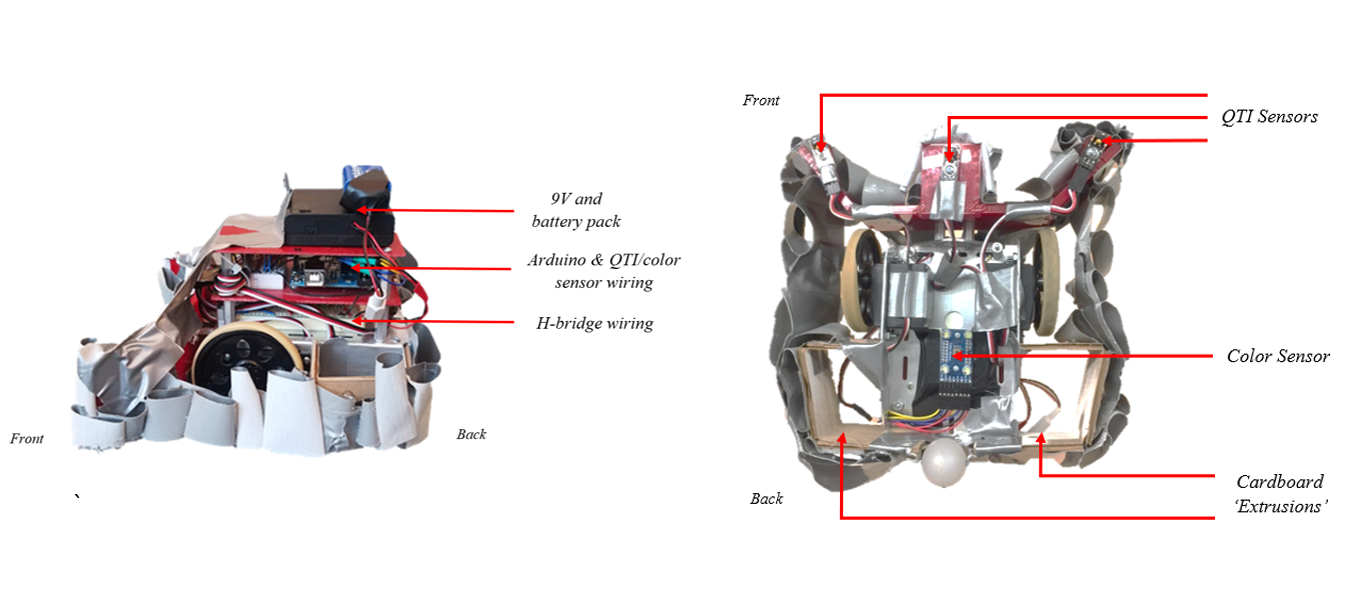
\includegraphics[scale=1.7]{Images/product2}
\captionof{figure}{\textit{Build Diagrams | Side View (L), Underside View (R)}}
\end{center}


\subsection{Bill of Materials}
\begin{center}
\begin{tabular}{ |c|c|c|c|c| } 
\hline
Part & Source & Individual Price & Quantity & Total Price\\
\hline
Acrylic Sheet & Scrap & \$5.00 & 1/4 of 8"x8" sheet & \$1.25\\ 
\hline
Cardboard & Scrap & \$0.25 & 2/3 of 6"x6" sheet & \$0.17\\
\hline
Duct Tape & Lab & free & 1/4 roll & free\\
\hline
\end{tabular}
\end{center}

\begin{center}
\textbf{Total: \$1.42}
\end{center}


\section{Software Design}

\subsection{Physical Route}
\begin{center}
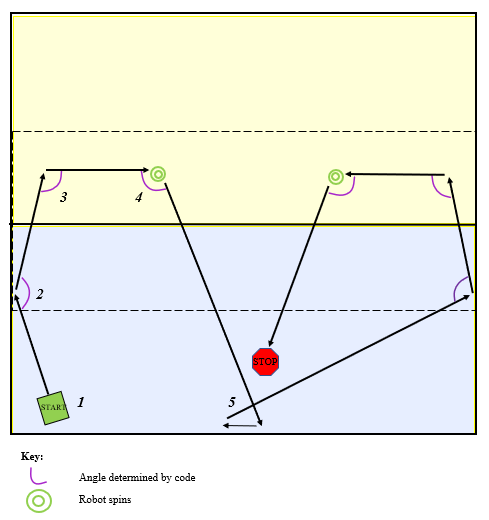
\includegraphics[scale=2.2]{Images/schematic}
\captionof{figure}{\textit{Route Schematic}}
\end{center}

\noindent
Referring to the above schematic, our strategy was as follows:
\begin{enumerate}
    \item Angle robot to ensure one QTI is triggered before the color border. Drive forward.
    \item Upon hitting the black line, turn a prescribed angle away from it.
    \item After passing the color border, turn to face oncoming blocks.
    \item Spin to collect any extra blocks and reorient to face our original side.
    \item Drive forward. Upon hitting the black line, back up to leave behind any blocks unattached to the tape.
\end{enumerate}

\noindent
\textit{*Complete a second loop on opposite half of the board, before stopping on our original side*}


\subsection{Logic}

\begin{center}
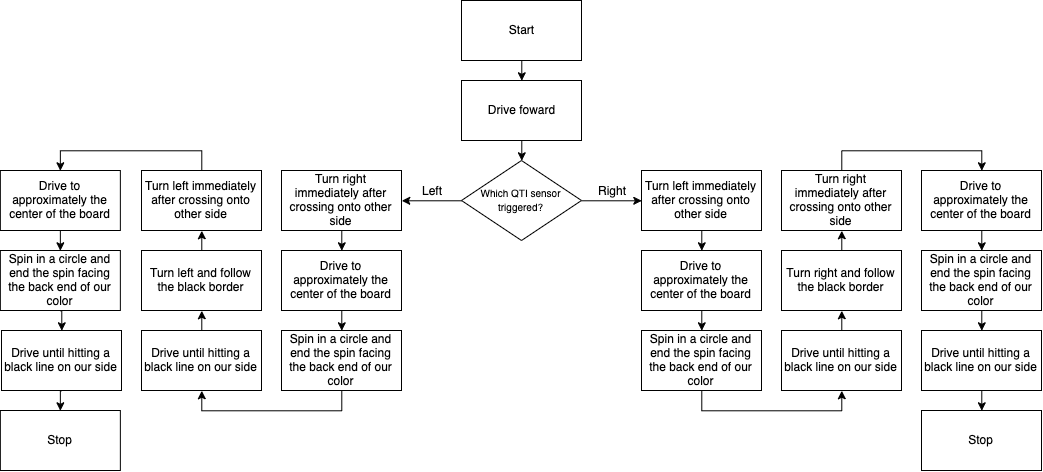
\includegraphics[scale=.41]{Images/flowchart.png}
\captionof{figure}{\textit{Algorithm Flowchart}}
\end{center}

\section{Discussion}
\subsection{Strengths and Weaknesses}
\textit{Simple mechanics, robust algorithm:}   Our robots greatest strength was its simplicity. Using tape as our block-collecting innovation proved to be a successful design choice not only because it consistently collected over half of the blocks, but also because it required no moving parts. Consequently, our manufacturing phase was short, we moved through checkpoints quickly, and we had ample time to test. This allowed us to troubleshoot many of the corner cases in our algorithm prior to the competition, resulting in victories against robots that were more mechanically clever. While other teams faced unexpected errors on competition day (randomly stopping, getting a wheel stuck on the edge of the board, becoming trapped in a corner, driving straight off the board and making no attempt to return, etc.), we spent our last week doing nothing but systematically discovering and eliminating unwanted behaviors. By the day of the competition, we had tested our robot so many times that we were certain it would drive its course regardless of starting position, variability in starting angle, deformations in the board, ambient lighting, and block interference, which put us at an advantage over other teams. We were also certain that it would not stop running its algorithm until it returned to the correct side, even if the other robot interfered with our loop pattern.
\\*

\noindent
\textit{Robot interference, self-destruction:}   Early on, we decided that aside from the most basic of interactions, accounting for robot interference would complicate our model far past the point of practicality given our time constraints, thus eliminating the use of sonar. That said, our tape design was inherently interactive. It was almost impossible for our robot to brush past or work its way around the opponent - any sort of collision would end in sticking and dragging. All we could do was hope that it was our robot doing the dragging, and not the other way around. This turned out to be true for a little over half the matches, likely because our robot had a low center of gravity. Most teams had higher centers of mass (risking instability) and long deployable arms, which gave us a large moment arm to push against. In the end, though, the results of these collisions were largely just a matter of luck. Even if we managed to drag the other robot, the additional weight meant that there was no guarantee we would make it back to our side in time. Due to this inconsistency, our robot\textquotesingle s successful tape strategy was also the source of its weakness. 
\\*

\noindent
\textit{Short-lived effectiveness:} Tape was an effective strategy for the purposes of this competition; however it is important to note that tape quickly loses its adhesive power over time. Too much longer and the tape would have been rendered completely ineffective. We took advantage of the knowledge that we would only be competing in several hours of competition, but increased gameplay time would have eventually neutralized our strategy. 

\subsection{Competition Performance}
During the round robin, we lost two rounds and won three rounds. This qualified us for the elimination bracket, during which we won our first match and lost in the quarterfinals. Two of our three losses could be attributed to a single issue: sticking to the other robot and being unable to drive back to our original side in time. Frustratingly, each time this happened, we had already collected at least half of the blocks and were on our second, auxiliary lap when we became stuck. We observed two different failure modes associated with robot contact:
\begin{enumerate}
    \item If we made full contact with a more powerful robot, we would get pushed to the opponent$'$s side with no chance of escape. This resulted in one of our losses. 
    \item If a collision resulted in only minimal contact, we were usually able to detach from the other robot. However, because our code did not account for such delays, our robot was knocked off it$'$s course and could take too long returning to the correct side. This resulted in another one of our losses.
\end{enumerate}

\noindent
Our third loss can simply be attributed to tape dragging on the ground. We had not accounted for the position of the tape to be altered by the weight of the blocks or collisions with other robots. In one match, the tape only momentarily stuck one side of the robot to the ground. However, this affected the robot$'$s path since the wheels were still turning; it veered off-course and was unable to make it back to our side in time. 

\subsection{Future Improvements}
\noindent
To mitigate the risk of being attached to another robot and unable to return to our own side, we should have programmed the robot to complete just one lap around the board rather than two. This would have still allowed us to collect over half of the blocks while lowering our risk of colliding with another robot. In fact, during gameplay, it was the second lap that resulted in several losses. For the loss due to tape dragging on the ground, simply accounting for the tape$'$s position being altered would have resulted in an additional victory. 

\section{Conclusions}

Our team was able to win a total of four matches: three in the round robin and one in the elimination bracket. Ironically, using tape proved to be both our greatest strength and greatest weakness. As far as collecting blocks went, the tape was extremely effective - in almost every match, our robot retained over half the blocks. However, getting stuck to our opponent and being unable to return to our side in time became a recurring issue. When such losses occurred, our efficient block-collecting strategy ended up benefiting the opposing team. 
\\*

\noindent
During the course of the project, we realized that when faced with a severe time restriction, keeping mechanical designs simple was paramount. Planning ahead, staying realistic, and allocating time for testing was the winning strategy for this competition. Retrospectively, we should have also applied this mindset to our movement algorithm by only performing one lap. 
\\*

\noindent
Overall, this project helped us bridge the gap between electrical, software, and mechanical systems. By learning the basics of coding and electronics, we will become better multidisciplinary communicators, and therefore better engineers. 


\newpage

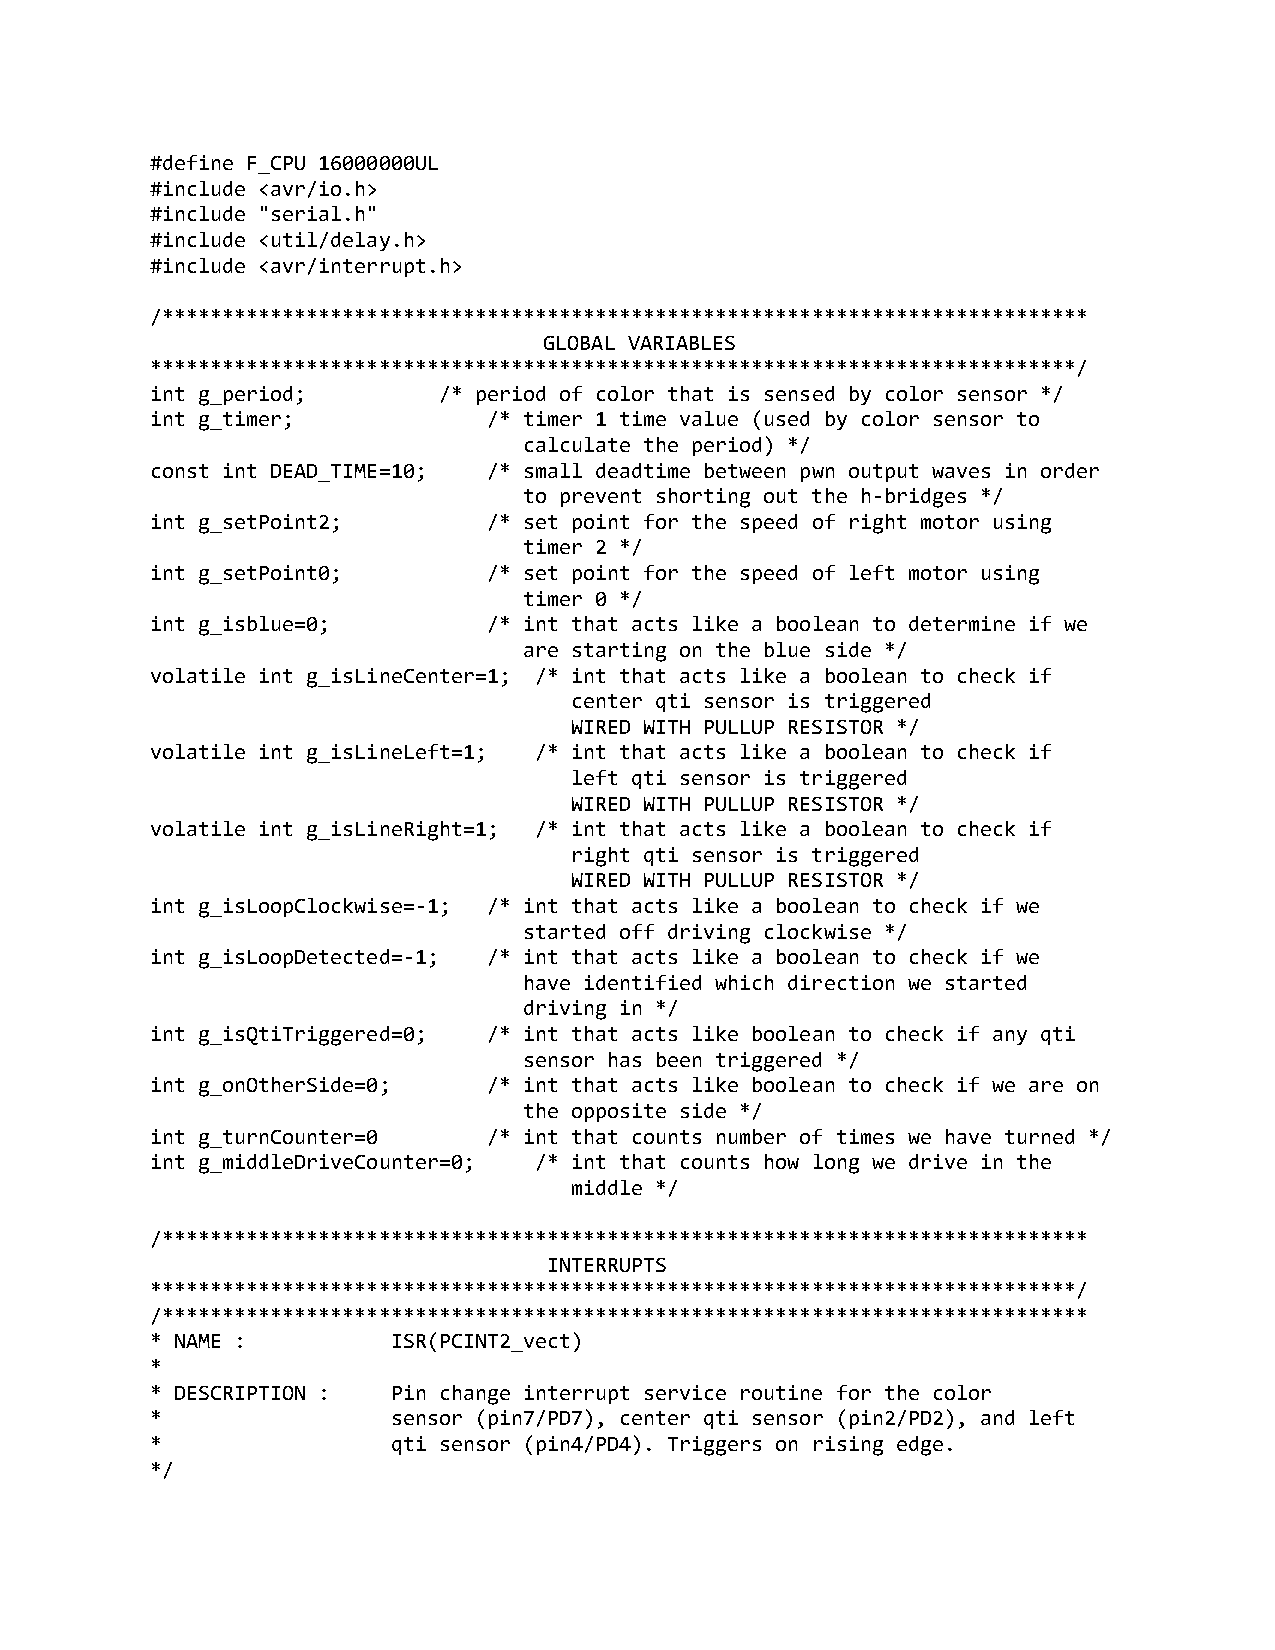
\includepdf[scale=1,pages=1,pagecommand=\section{Appendix}\subsection{Code}]{code}
\includepdf[scale=1,pages={2-}]{code}
\subsection{H-Bridge Schematic}

\begin{center}
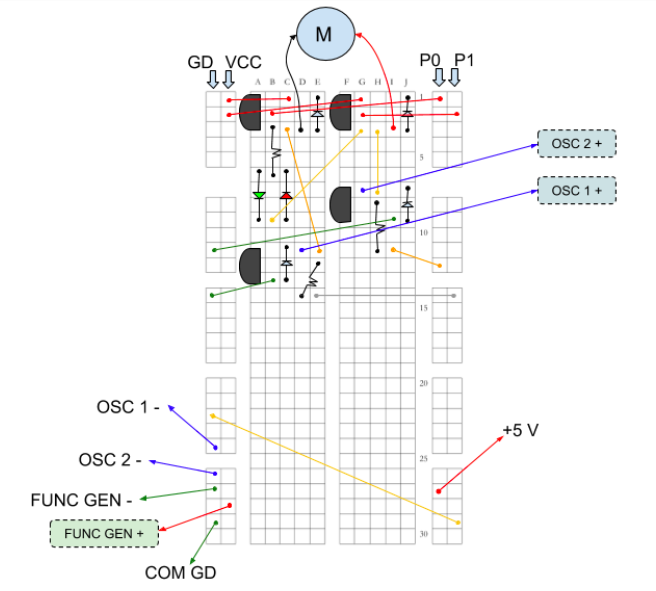
\includegraphics[scale=.7]{Images/hbridge.png}
\captionof{figure}{\textit{Marigot's Lab 4 H-Bridge}}
\end{center}

\end{document}


